% -%-%-%-%-%-%-%-%-%-%-%-%-%-%-%-%-%-%-%-%-%-%-%-%-%
% PIM380                                           % 
% Data:28/06/2013                                  %
% Paris,France                                     % 
% Groupe:                                          %
% - Tiago Chedraoui Silva                          %  
% - Vinicius Dias Gardelli                         %
% -%-%-%-%-%-%-%-%-%-%-%-%-%-%-%-%-%-%-%-%-%-%-%-%-%

\documentclass[a4paper,11pt]{article}

\usepackage[francais,listings,algo]{pim}

\usepackage[version=3]{mhchem}
\bibliographystyle{apalike}  

% Cover %
\def \ttprofname{Prof \textordmasculine.~Dr \textordmasculine.Tamy Boubekeur} % teachers name
\def \ttabrv{PIM380 } % abbreviation of names class
\def \ttabrvxt{} % period
\def \mytitle{Reconstruction 3D temps-réel HD de visages} % Big title
\def \ttauthi{Tiago~Chedraoui~Silva} % author's name
\def \ttxti{Casier: 361 } % Extra text right side of name
\def \ttauthii{Vinicius~Dias~Gardelli} % author's name
\def \ttxtii{Casier: 379 } % Extra text right side of name
\def \ttdate{Juillet 25, 2013} % date

\spc{1.5}
\begin{document}
\thispagestyle{empty}
\titleTMB 
 % \begin{titlepage}
 % \thispagestyle{empty}
 % \begin{center}  \begin{figure}[h!]
 %   \begin{center}
 %     
\includegraphics[scale=0.1]{img/logo.jpg}
 %   \end{center}
 % \end{figure}
 %\end{center}
 % %\vspace{0.3cm}
 % \begin{center} 
 %   {\Large \textsc{Reconstruction 3D temps-réel HD de visages}} 
 %   \\\vspace{0.5cm}
 %   {\textsl{Rapport Projet PIM - Projet d’Innovation Master}}
 %   \\\vspace{1cm}
 %   \begin{tabular}{rl}
 %     \textbf{Elève}:       & \ttauthi \\
 %     \textbf{Elève}:       & \ttauthi \\
 %     \textbf{Professeur}: & \ttprofname
 %   \end{tabular}
 %   % Instituto de computação\\
 %   \vspace{0.5cm}
 %   \\ \ttdate     
 % \end{center}
 % \vspace{0.5cm}
%  \begin{abstract}
%    Dans les deux décennies, les animations faciales ont eu plusieurs aproches. Actuellment, les dernières méthodes sont basée sur une capture passive dont la configuration est presque entièrement automatiques. 
%    Le but de ce projet est de réproduire une reconstruction 3D de visages à travers d'une méthode de capture passive qui utilisera que des outils périphériques peu coûteux, qui sont plus accessibles à la majorité des personnes.
 % \end{abstract}
  % Sumário
%\tableofcontents

%\end{titlepage} 

\newpage
\thispagestyle{empty}
  \begin{abstract}
    Dans les deux décennies, les animations faciales ont eu plusieurs aproches. Actuellment, les dernières méthodes sont basée sur une capture passive dont la configuration est presque entièrement automatiques. 
    Le but de ce projet est de réproduire une reconstruction 3D de visages à travers d'une méthode de capture passive qui utilisera que des outils périphériques peu coûteux, qui sont plus accessibles à la majorité des personnes.
 \end{abstract}

\newpage
\thispagestyle{empty}
\tableofcontents
\newpage
\setcounter{page}{1}

\section{Introduction}

Les animations faciales ont eu plusieurs aproches dans les deux décennies. Les dernières méthodes sont basée sur une capture passive dont la configuration est presque entièrement automatiques [Bradley et al. 2010; Popa et al. 2010]. 

Cependant, une technique pour capturer des performances expressives très détaillées qui évite détérioration avec le temps doit encore être réalisé.

L'objectif du projet est la recherche et la mise au point d'un algorithme de reconstruction 3D de surface dynamiques appliqué spécifiquement à un visage. 

Les données d'entrées sont provienues d'une kinects.

\section{Etat de l'art}

Les animations faciales a eu plusieurs approches dans les deux décennies, 
parmi eux: l'utilisation des modèles de visage qui sont ajustent aux images, 
l'utilisent de l'éclairage actif et utilisent des marqueur.

En vue d'avoir une méthode moins coûteux et intrusif, les dernières méthodes sur les animations faciales sont basée sur une capture passive.

% dont la configuration est presque entièrement automatiques.   [Bradley et al. 2010; Popa et al. 2010]. 

Dans cette section, nous aurons une bref description de chaque approche.

\subsection{Ajuster les faces aux images}
Une approche pour la capture des faces est de commencer avec un modèle de visage déformable, puis de déterminer les paramètres qui correspondent le mieux au modèle des images ou des vidéos d'un acteur performant.

Un inconvenient de cette approche est qu'il exige un grande nombre de calculs et pour qu'il soit traitable, le modèle de visage doit être d'une faible résolution.
Comme résultat, il n'est généralement pas possible d'obtenir les détails les plus fins qui sont responsables pour les expressions et réalisme de la scene.

De plus, le visage déformable a tendance à être très générique, de sorte que les animations résultant souvent ne ressemblent pas à l'acteur capturé.

\subsection{Marqueurs et éclairage actif}

Une autre approche commune pour la capture d'une scene est l'utilisation des marqueurs placés à la main ou de la peinture pour le visage.

Ces technique peuvent produire un suivi robuste des performances très expressifs et sont généralement adaptés à une variété de conditions d'éclairage.

Cependant, un inconvenient de l'utilisation des marqueurs est le coût de les placer manuellement, ainsi comme la caracteristique invasive de la technique. De plus, pour acquerir la couler de la visage ou de la texture, ces marqueurs doievent être retirés.

En outre, cette méthode présent aussi l'inconvenient de fournir une résolution limitée, car la capture à une échelle des pores n'a pas été démontré avec cette approche.

Une alternative à placer des marqueurs sur le visage est de projeter un éclairage actif sur le sujet. D'une part, cette approche nécessite moins de la configuration manuel, mais il continue à être envahissant et constitue encore un problème pour la acquisition de la couleur.

\subsection{Capture passive }

Les recherches plus récents s'ont concentrées sur la reconstruction passive, c'est-à-dire, sans la nécessité de marqueurs, de la lumière structurée ou du matériel coûteux.

Les résultats obtenus par ce type approche sont très satifaisants, par exemple la reconstituitions de la géométrie du visage a uné échelle des pores a été déjà réalisé.

Cependant, il reste encore des improvements pour cette approche, notamment par rapport à la propagation de la maillage de points d'une trame à autre.

\section{Le projet}

Dans ce projet, on essayera de réproduire les étapes réalises par Beeler et al. dans le papier ``High-quality passive facial performance capture using anchor frame'' pour la création d'une mesh qui réproduit la visage.
Dans l'article sont matériel est un matériel d'haute définition, notre but dans le projet est de réaliser, ainsi que possible, une version moins chères de la création des visages, qui pourrait etre réalisé par toutes les personnes disposant d'une limitation matériel.

\subsection{Matériel}

Ci-dessous la liste de matériel utilisé dans le projet: 

\begin{itemize}
\item Une Kinect responsable pour captures des images 640 × 480 en couleur 32 bits ainsi comme une image de profondeur. 
\end{itemize}

\begin{figure}[h!]
  \begin{center}
    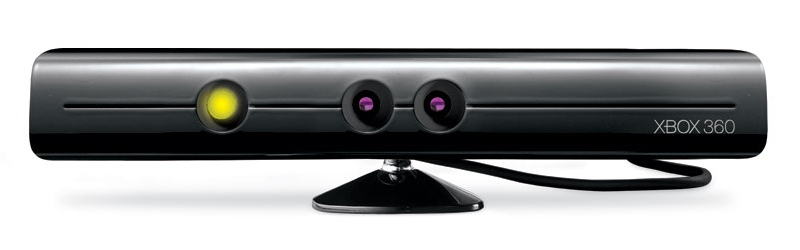
\includegraphics[scale=0.2]{img/kinect.jpg}
    \caption{Kinect - Dispositif utilisé pour la capture des images}
  \end{center}
\end{figure}

\subsection{L'environnement de travail}

Le projet est développé sous un système d'exploitation linux, en utilisant un système de contrôle de version git (https://github.com/tiagochst/PIM2013). 
De plus, les librairies externes utilisés sont: Eigen, OpenNI et possiblement OpenCV dans l’avenir.

Pour la compilation du projet on a décidé d’utiliser l’outil qmake pour une génération des Makefiles pour faciles et aussi intégré avec le framework qt. 
Pour cela les fichiers suivants ont été crées: PIM380.pro. 

Par ailleurs, pour avoir un suivi plus visuel de l’état du projet on utilise un outil en ligne pour la création d’un kanban(http://kanbanize.com/) dont l’objectif est d’afficher la situation actuel du projet. Ainsi, le kanban peut vous montrer ce qui est en train d’être fait, ce qui a été fait, ce qui doit être fait, les tests à faire et les bugs à traiter qui ont été trouvés.

Finalement, pour la création de la documentation du code du projet, le logiciel doxygen a été utilisé. 


\subsection{Méthodes}

Le projet est divisé en cinq étapes: 

\begin{enumerate}
\item Calcul du maillage initial
\item Ancrage
\item Localisation image-space
\item Propagation de la maillage
\item Raffinement de maillage
\end{enumerate}

\begin{figure}[h!]
  \begin{center}
    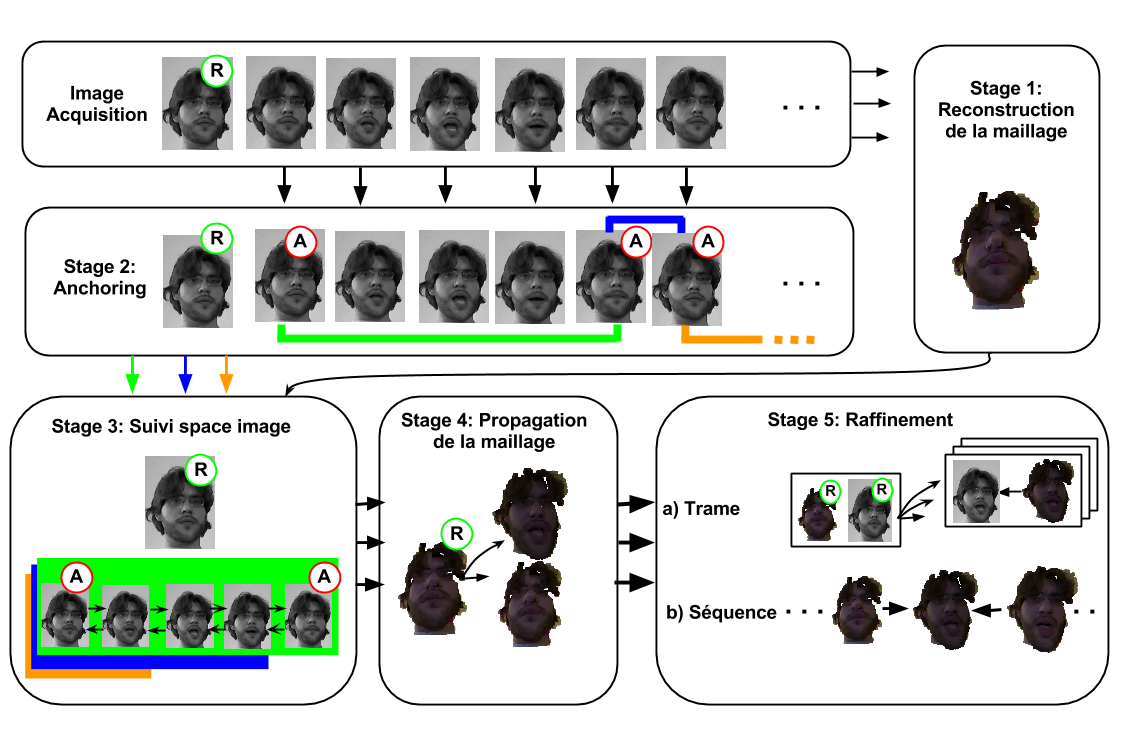
\includegraphics[scale=0.4]{img/projDiagram.png}
    \caption{Etapes du projet}
  \end{center}
\end{figure}

\subsubsection*{Calcul du maillage initial}
Chaque image de la séquence est traitée indépendamment pour générer une première estimation de la maillage pour cette trame.

\subsubsection*{Ancrage}
Une trame est identifié manuellemnt comme la trame de réference. Puis, les trames qui ont une apparance similaire (expression du visage samblable et l'orientation de la tête) sont identifiées automatiquement et étiquetés comme des trames d'ancrage. Ces trames ancres seront un moyen de partitionner la séquence complète des clips de trames pour le traitement dans la prochaine étape.

\subsubsection*{Localisation image-space}
Le but de cette étape est de suivre les pixels de l'image à partir du trame de référence pour chaque image dans la séquence. 

Le processus commence par le suivi de pixels d'image à partir de la trame de référence pour les trames d'ancrage, ce qui est simple, car l'aspect de l'image en deux trames est, par définition, similaire. Cela permettra d'orienter le cheminement de pixels d'image à partir de la trame de référence à toutes les autres trames dans la séquence. 
Le suivi des trames non ancres est réalisé de manière séquentielle, à partir des trames ancres les plus proches.

\subsubsection*{Propagation de la maillage}

Une propagation de maille désigne le calcul de nouvelles positions des sommets du maillage dans l'espace, en correspondance avec le mouvement physique de la face.

Un moyen pour propager la la maillage de référence (maillage de la trame de référence calculé à l'étape 1), pour toutes les trames dans la séquence, est l'utilisation des pixels de l'image suivis obtenues à l'étape 3.
 
\subsubsection*{Raffinement de maillage}

Les étapes précédentes ont généré une propagation de la maille de référence pour chaque trame dans la séquence. Cette séquence de maillage déformant fournit une estimation initiale du mouvement du visage, ce qui est raffiné pour garantir la cohérence avec les données d'image en appliquant priori sur la cohérence spatiale et temporelle de la surface déformée.


\section{Les étapes de développement}
\subsection*{Interface Kinect}

Un des objectives du projet est d’avoir une interface avec la Kinect pour capturer les images nécessaires pour la reconstruction faciale.

Pour qu’on puisse accéder aux données du dispositif Kinect, l’API OpenNI a été utilisé. Cette API fournit des interfaces de communication qui interagissent à la fois avec les capteurs et les composants intermédiaires, qui analysent les données provenant des capteurs.

La Kinect nous fournit une image RGB et sa profondeur en niveaux de gris dans une résolution VGA (640×480).

Actuellement, quand la fonction de la caméra est appelée, on accédera aux données de la Kinect et on dessinera par défaut la carte de profondeur par dessus de la carte graphique. 

%Pour une interaction, les actions suivantes sont possibles: 

% tabela

%La sortie peut être vue ci-dessous:

%*Figure 1: Carte de profondeur
%*Figure 2: Image

\subsection*{Interface graphique}

Pour la visualisation des images et des objets 3D, une interface graphique crée en utilisant le framework QT et la librairie QGLviewer. 

Nous avons utilisé l’outil Pencil pour faire une maquette de l’interface. Ci-dessous, la maquette pour la visualisation de déplacements entre deux frames.

Le résultat en utlisant le framework Qt peut être vu, ci-dessous.

Pour la sélection des  frames ancres on a deux interfaces, une pour la sélection manuel et l’autre pour la sélection automatique. Les images de l’interface sont ci-dessous:

Sélection d'ancres manuellement: 

\begin{figure}[h!]
  \begin{center}
    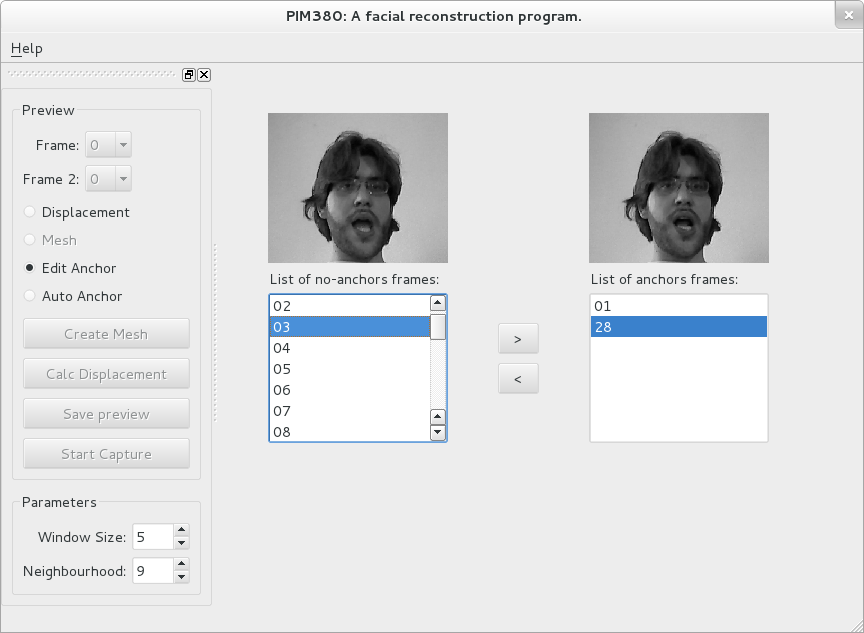
\includegraphics[scale=0.4]{img/editAnchorList.png}
    \caption{Edition de la liste des ancres}
  \end{center}
\end{figure}

Sélection d'ancres automatiquement:

\begin{figure}[h!]
  \begin{center}
    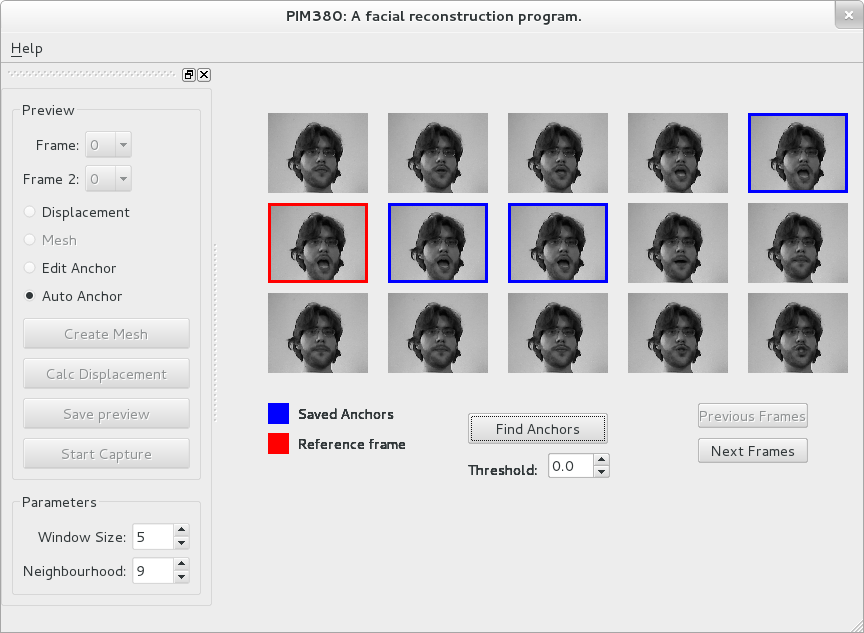
\includegraphics[scale=0.4]{img/AnchorAutomaticSelection.png}
    \caption{Séléction automatique des ancres. Entrée: trame de référence (rouge) et seuil. Sortie: trames ancres (bleau)}
  \end{center}
\end{figure}


\subsection{Correspondance des pixels}

Pour la correspondance des pixels entre deux images, on évalue utilise un algorithme basée sur la valuer de la intercorrélation normalisée calculée sur une fenêtre carrée (3x3). La valeur la plus haute est notre meilleur correspondance.

D'abord, le Pixel $p$ dans l'image $I$ est comparé à tous les pixels dans l'image $J$ dans une zone de recherche donné, et la meilleure correspondance est conservée. 

Après avoir la meilleur correspondance, l'écart au pixel $p$ est calculé en utilisant les valeurs de la intercorrélation normalisée avec le point $p$ et ses deux voisins dans l'image $J$. En utilisant ses trois points, on utilisé un polynôme de degré deux pour trouver la valeur maximun que sera la valeur de la disparité.

Pour l'utilisation des piramides des images, la correspondance est calculée pour tous les pixels en utilisant les estimations de la disparité de la couche précédente pour limiter la zone de recherche. 

En suite, pour certifier la bonne correspondance entre les pixels, quelques constraintes on été implementées, pour validé la correpondance.
\begin{description}

\item[Lissage] Pour avoir une cohérence entre les voisins, plus de la moitié de tous les voisins dans une fenetre 3 x 3 diffèrent par un écart de moins d'un pixel de la disparité calculée au pixel $p$.  

\item[Unicité] la corresponce doit etre bijective, c'est-à-dire si le pixel $p$ dans l'image $I$ correspond au pixel $q$ dans l'image $J$, alors $q$ doit également correspondre à $p$. Pour cette constrainte une disparité d'un pixel est acceptè.
\item[Ordre] Disparité calculée au point $p$ ne dépasse pas la disparité de son pixel droit voisin par plus d'un pixel.
\end{description}

Pour les pixels qui ne remplissent pas ces contraintes, la correspondance sera rafait, mais cette fois, les estimations de la disparité des pixels voisins qui on remplit les contraintes seront utilisées. 

Le resultat de cette étape, est un map de disparité, contenant pour chaque pixel de l'image $I$, la valeur de displacement dans l'image $J$. 

\begin{figure}[h!]
  \begin{center}
    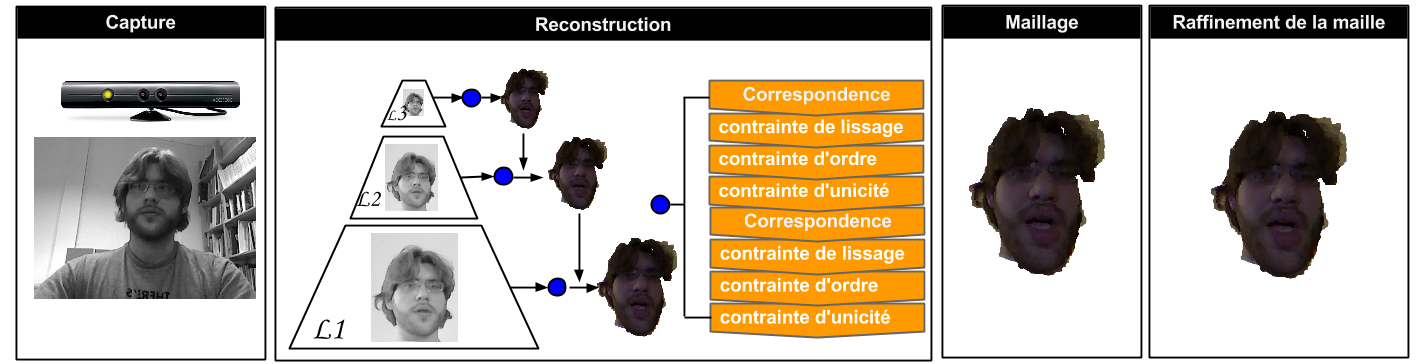
\includegraphics[scale=0.35]{img/projSystem.png}
    \caption{Le système proposé: de la capture à la reconstruction finale}
  \end{center}
\end{figure}


\subsection{Raffinement}

\section{Résultats}

\section{Conclusion}

\section{Remerciement}
Nous tiendrons tout d’abord à remercier Dr Tamy Boubekeur, le professeur responsable du projet et notre tuteur, de nous avoir accueilli comme élévés au sein du projet et la confiance qu’il nous a accordé tout au long de notre projet.

Nous remercions également Thierry Guillemot et Stéphane Calderon, pour leur volonté à m’aider pendant toute la période de notre projet PIM.

\nocite{Beeler:2010:HSC:1778765.1778777}
\nocite{Beeler:2011:HPF:2010324.1964970}

% ******************************************************
% REFERENCIAS BIBLIOGRÁFICAS
% ******************************************************
\begin{small}
  \bibliography{pim}
\end{small}
\section*{}

\end{document}
